%! Author = admin
%! Date = 2023/12/4

% Preamble
\documentclass[a4paper]{article}

% Packages
\usepackage[margin=1in]{geometry}
\usepackage[fontset=founder]{ctex}
\usepackage{anyfontsize}
\usepackage{graphicx}
\usepackage{amsmath}
\usepackage{amssymb}
\usepackage{mathabx}
\usepackage{multirow}
\usepackage{subfig}

\graphicspath{{../figures/}}

\title{\textbf{晶体管共射极单管放大器}}
\author{姚苏航\qquad PB22061220 \\ 庞宇乐\qquad PB22061166}
\date{实验时间: 2023年11月29日\qquad 座位号: 05}

% Document
\begin{document}
    \maketitle


    \section{实验目的}\label{sec:}

    \noindent{1.掌握放大器静态工作点的测量与调试方法。\cite{ed4}}

    \noindent{2.学习放大电路的交流特性等性能指标的测量方法。}

    \noindent{3.掌握静态工作点与输出波形失真的关系,了解最大不失真输出电压的测量方法。}


    \section{实验原理}\label{sec:10}
    \begin{center}
        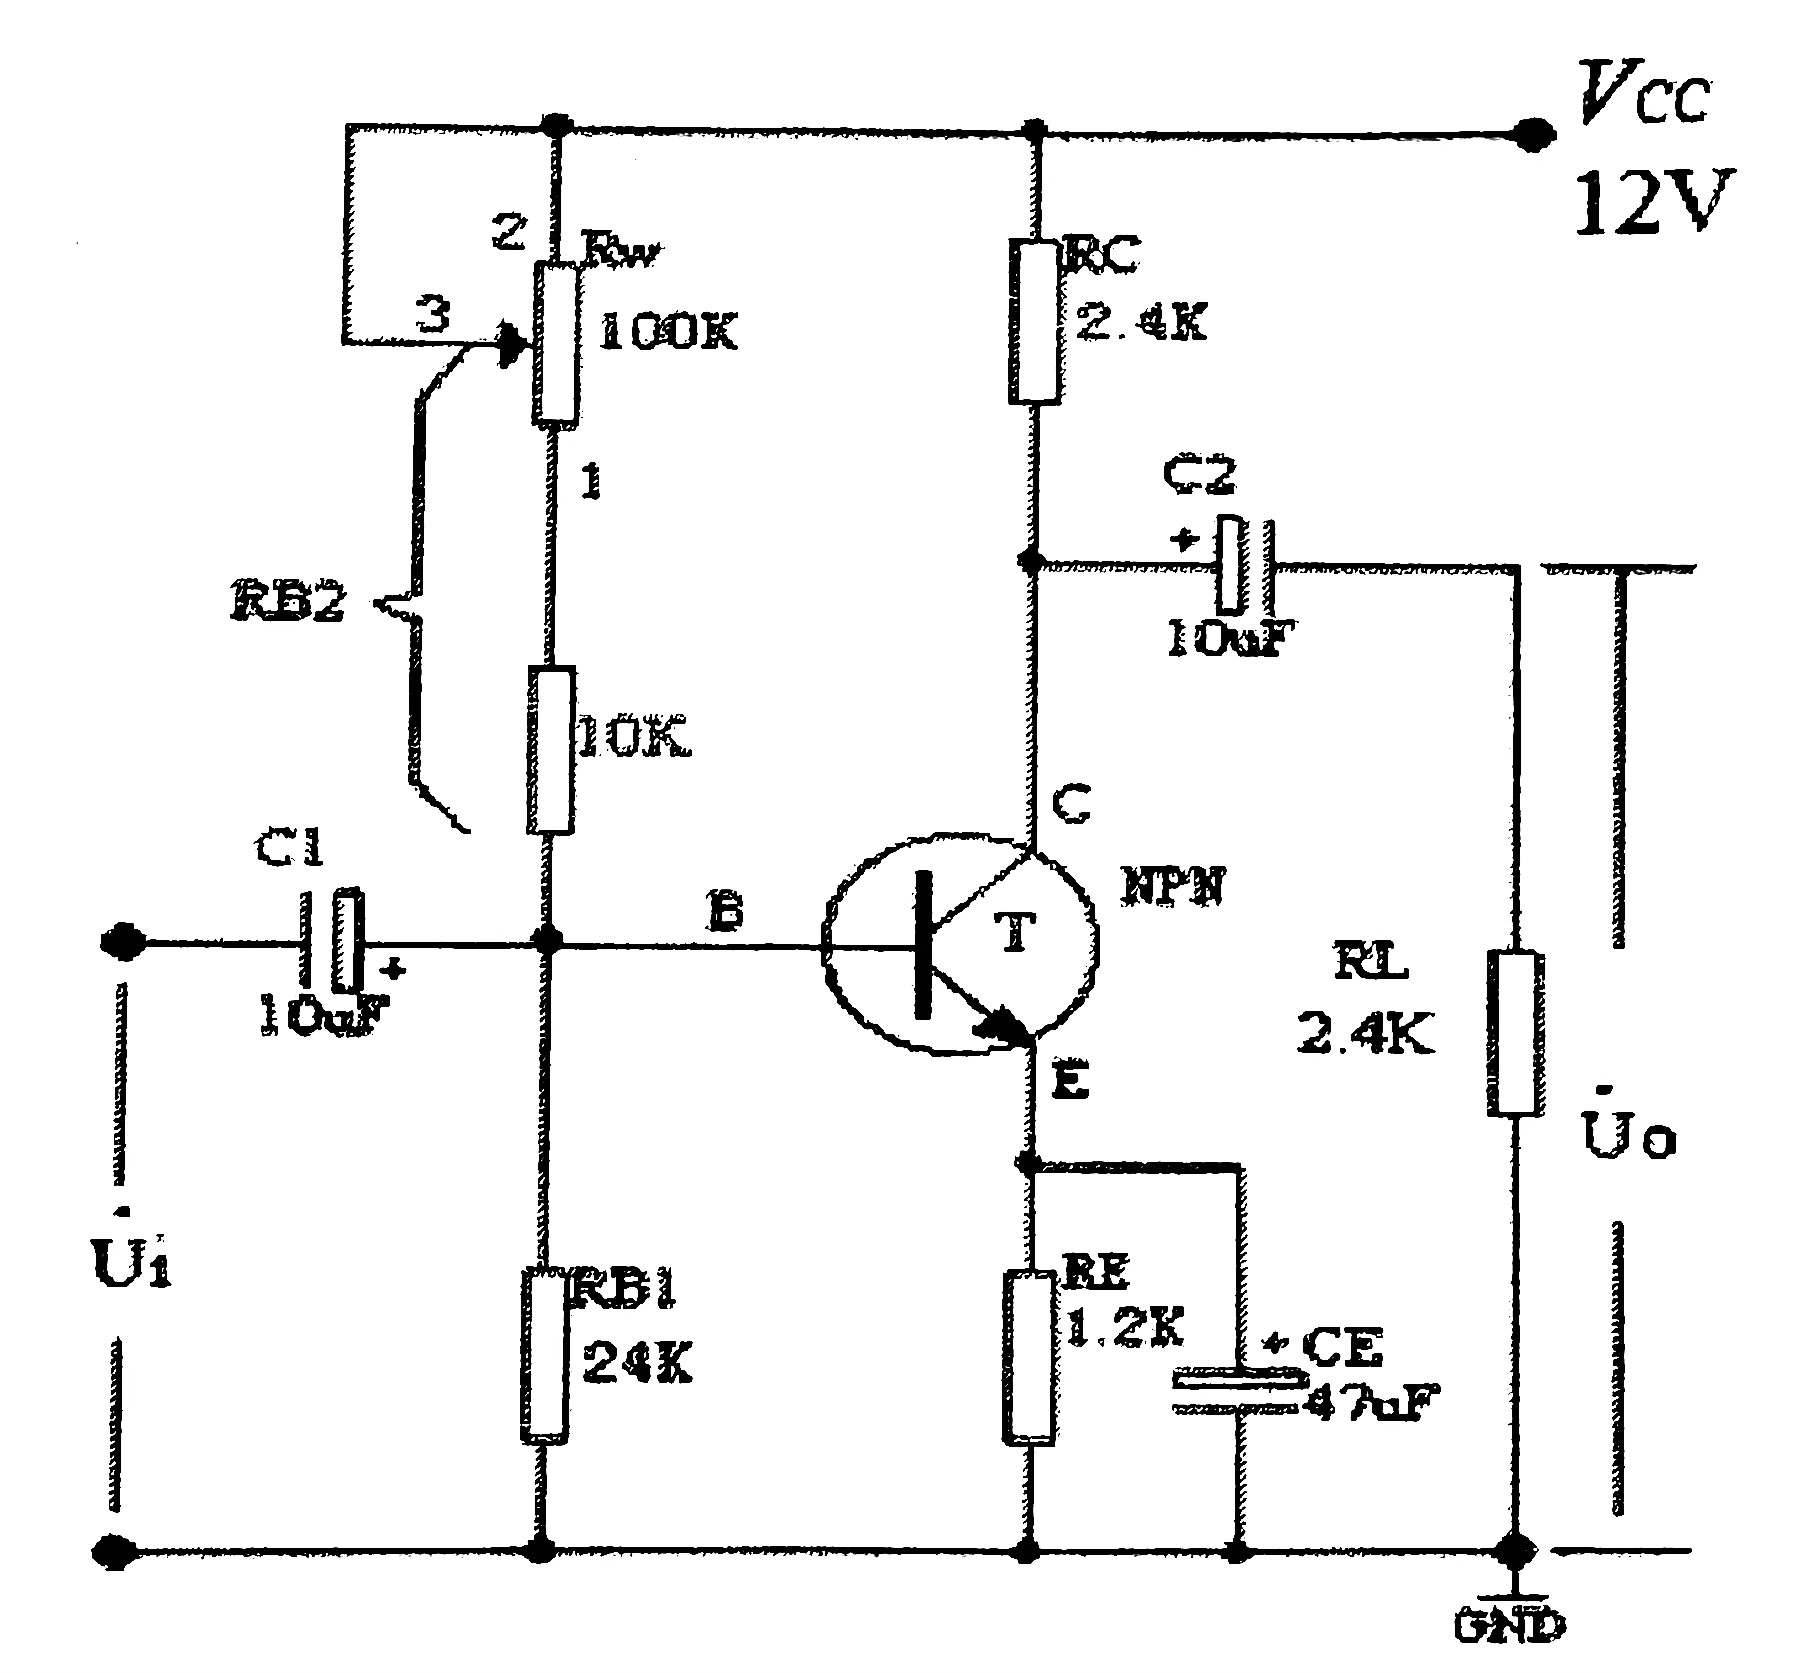
\includegraphics[height=150pt]{AC}\\
        {\small 图一:共射极单管放大电路}
    \end{center}

    {{图一为电阻分压式工作点稳定单管放大器实验电路图。其中偏置电路采用$R_{B1}$和$R_{B2}$组成的分压电路。$V_{CC}$作为集电极电源为电路提供能量,保证发射结正偏、集电结反偏。集电极电阻$R_C$将变化的电流转变成变化的电压,是电路具有电压放大能力。发射极电阻$R_E$引入负反馈稳定电路,稳定放大器静态工作点。耦合电容$C_1$和$C_2$隔离输入输出与电流直流的联系,同时能使信号顺利输入输出。}}


    \section{实验仪器}\label{sec:2}


    \section{测量静态工作点}\label{sec:3}

    \subsection{实验内容}\label{subsec:2}
    \begin{center}
        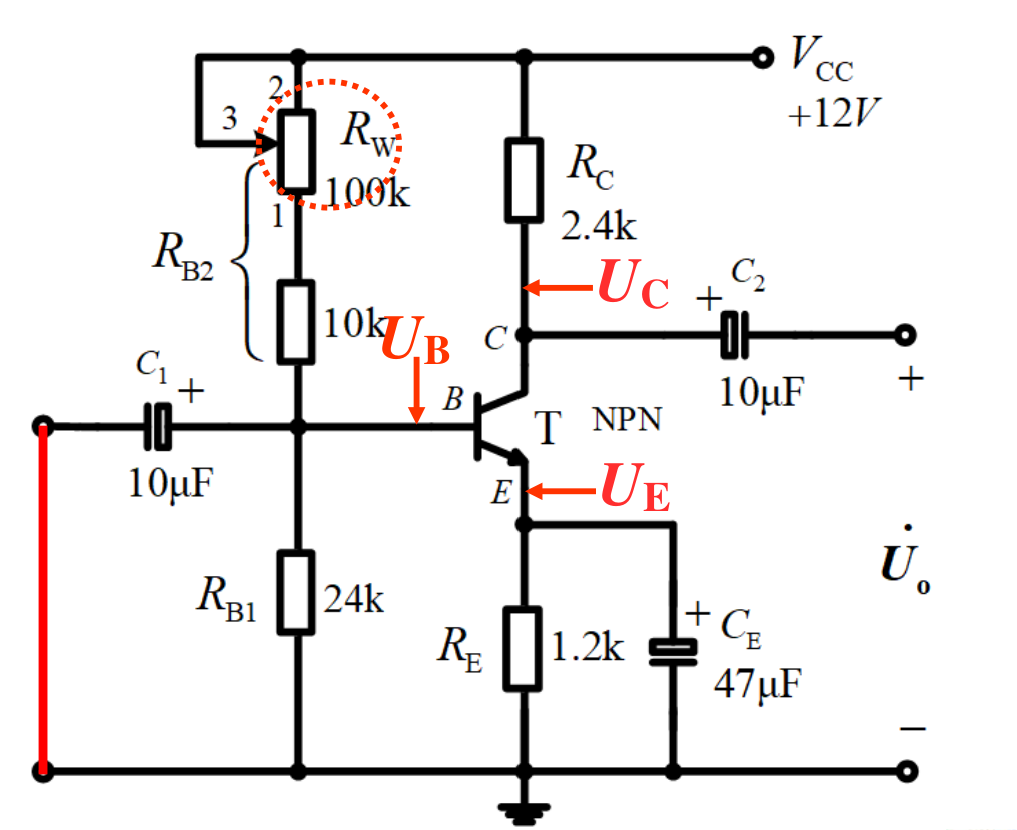
\includegraphics[height=150pt]{exp2}\\
        {\small 图二:实验电路}
    \end{center}

    \subsection{实验数据与误差分析}\label{subsec:3}

    \subsection{注意事项}\label{subsec:4}


    \section{测量电压放大倍数}\label{sec:4}

    \subsection{实验原理}\label{subsec:5}

    \subsection{实验内容}\label{subsec:6}

    \subsection{实验数据与误差分析}\label{subsec:7}
    \begin{center}
        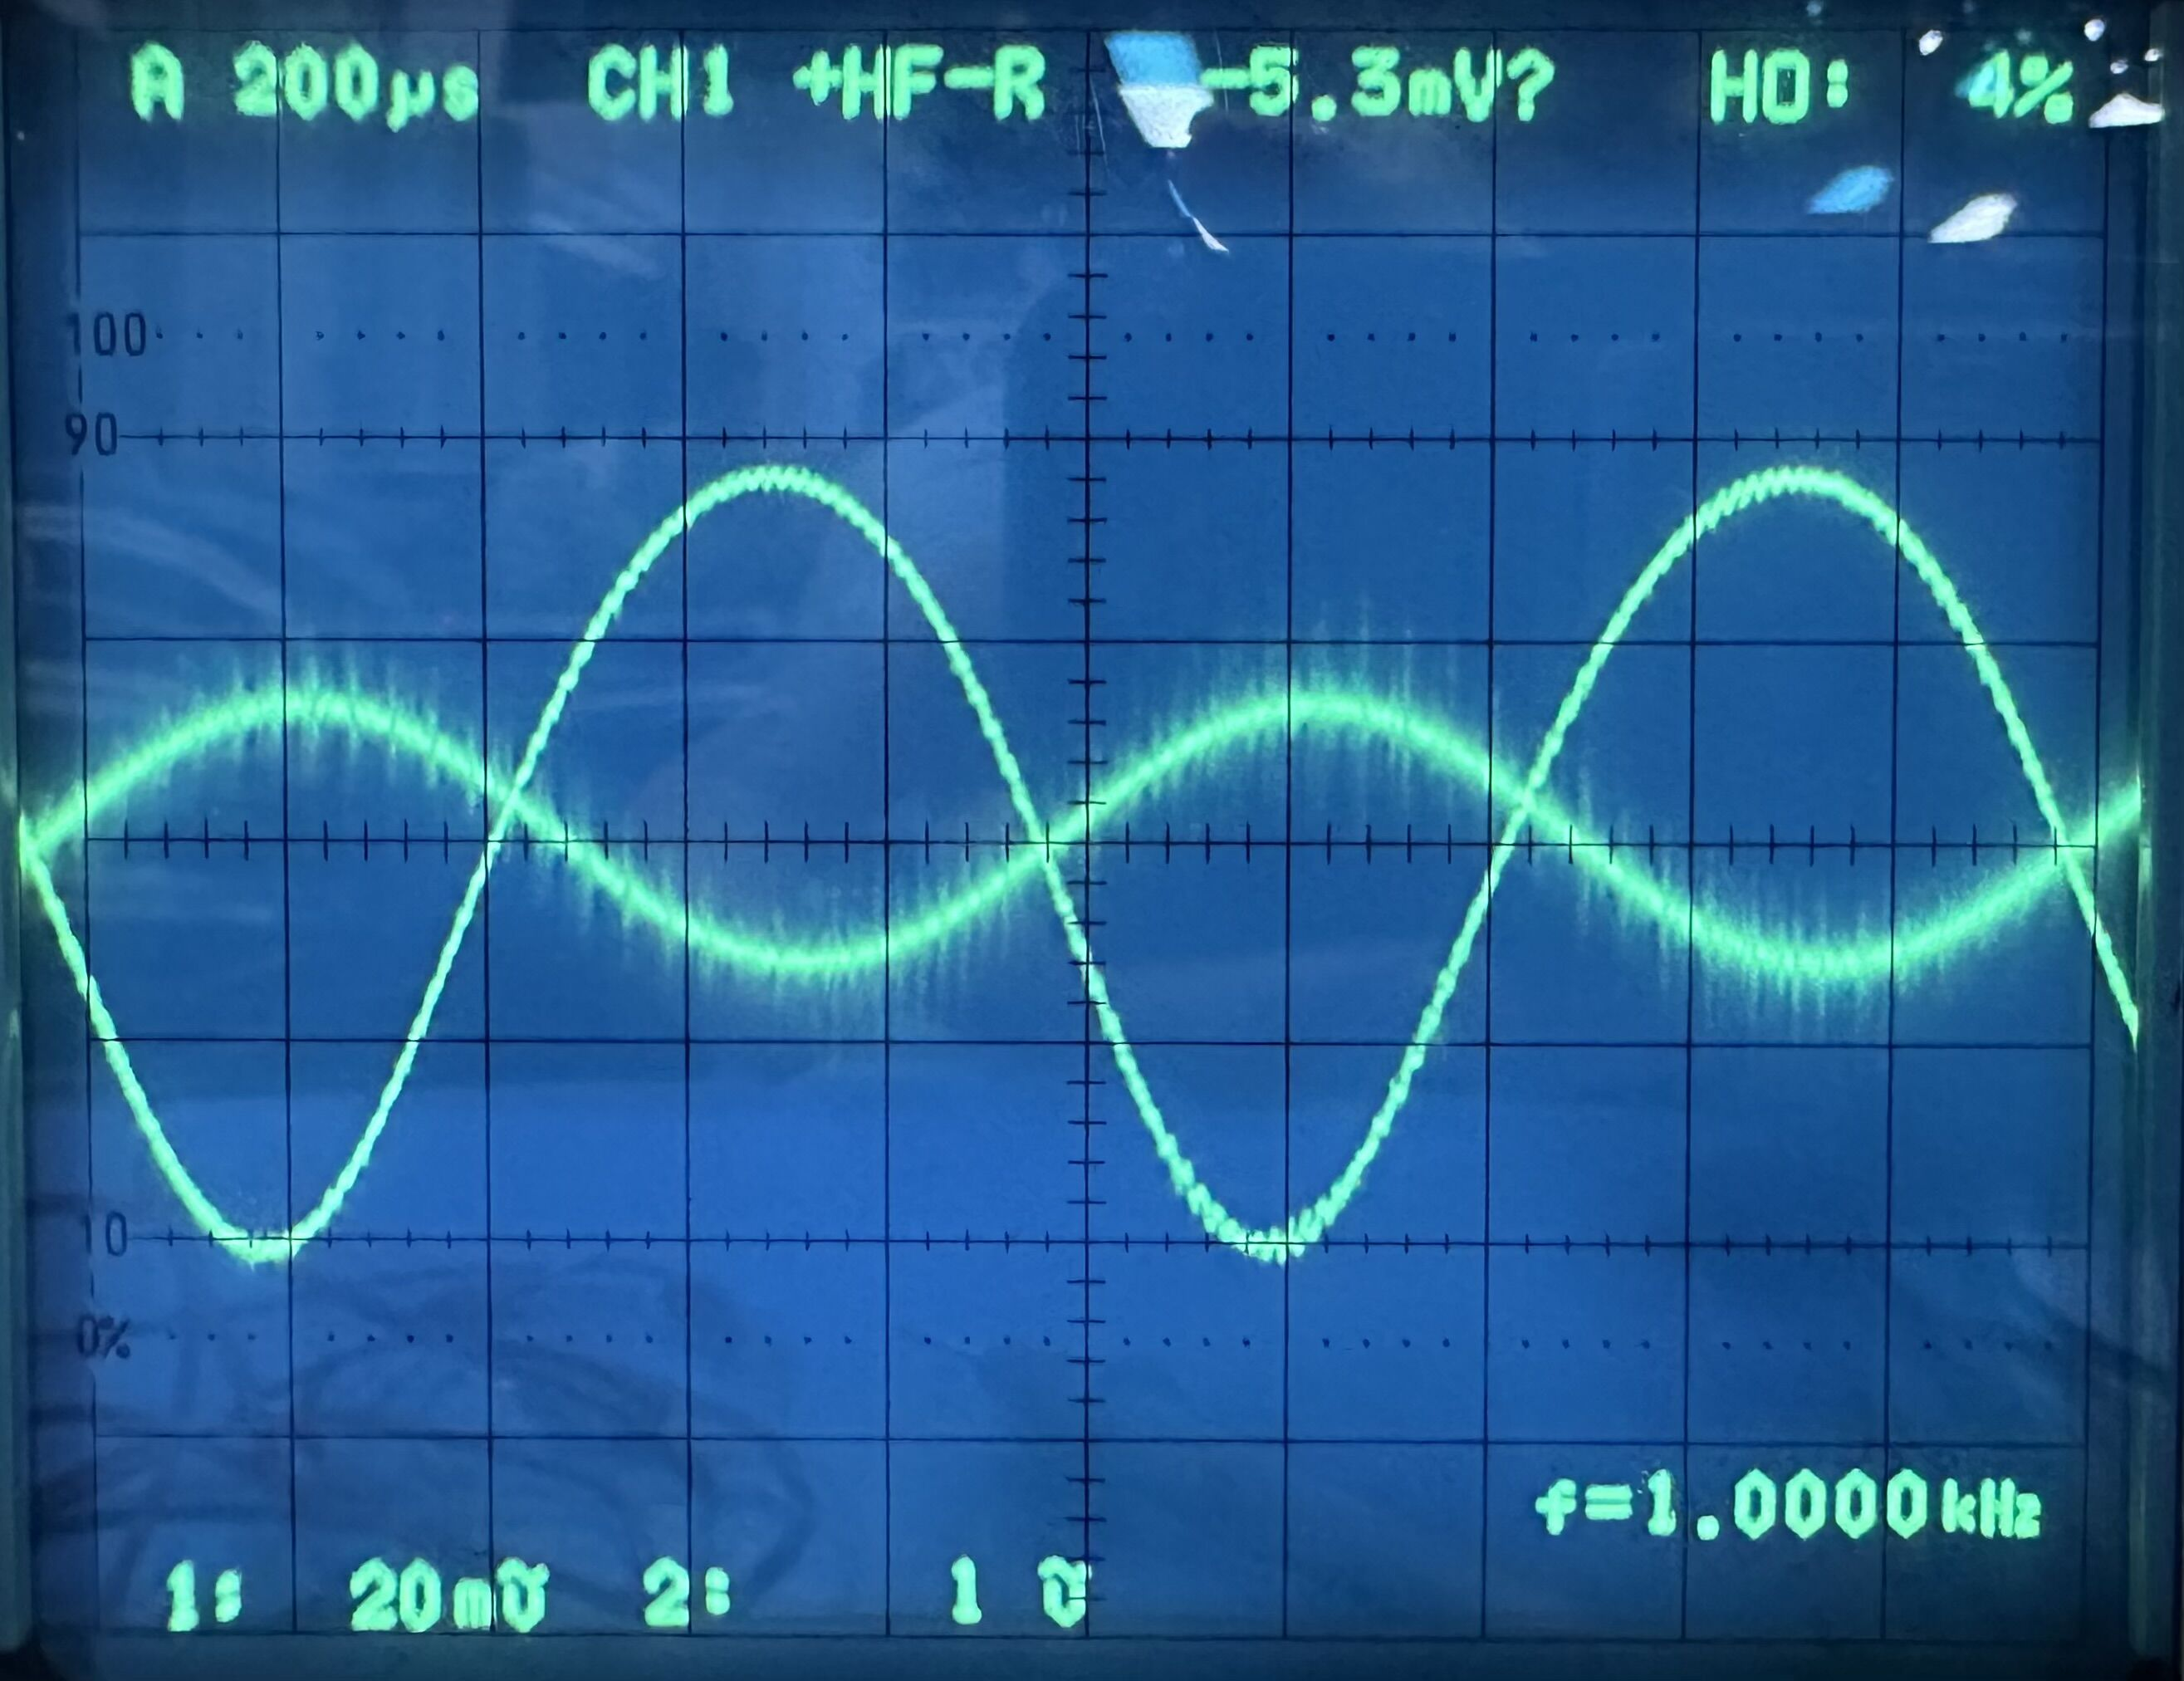
\includegraphics[height=130pt]{ref}\\
        {\small 图三:$u_o$和$u_i$的相位关系}
    \end{center}

    \subsection{注意事项}\label{subsec:8}


    \section{测量输入电阻和输出电阻}\label{sec:5}
    \begin{center}
        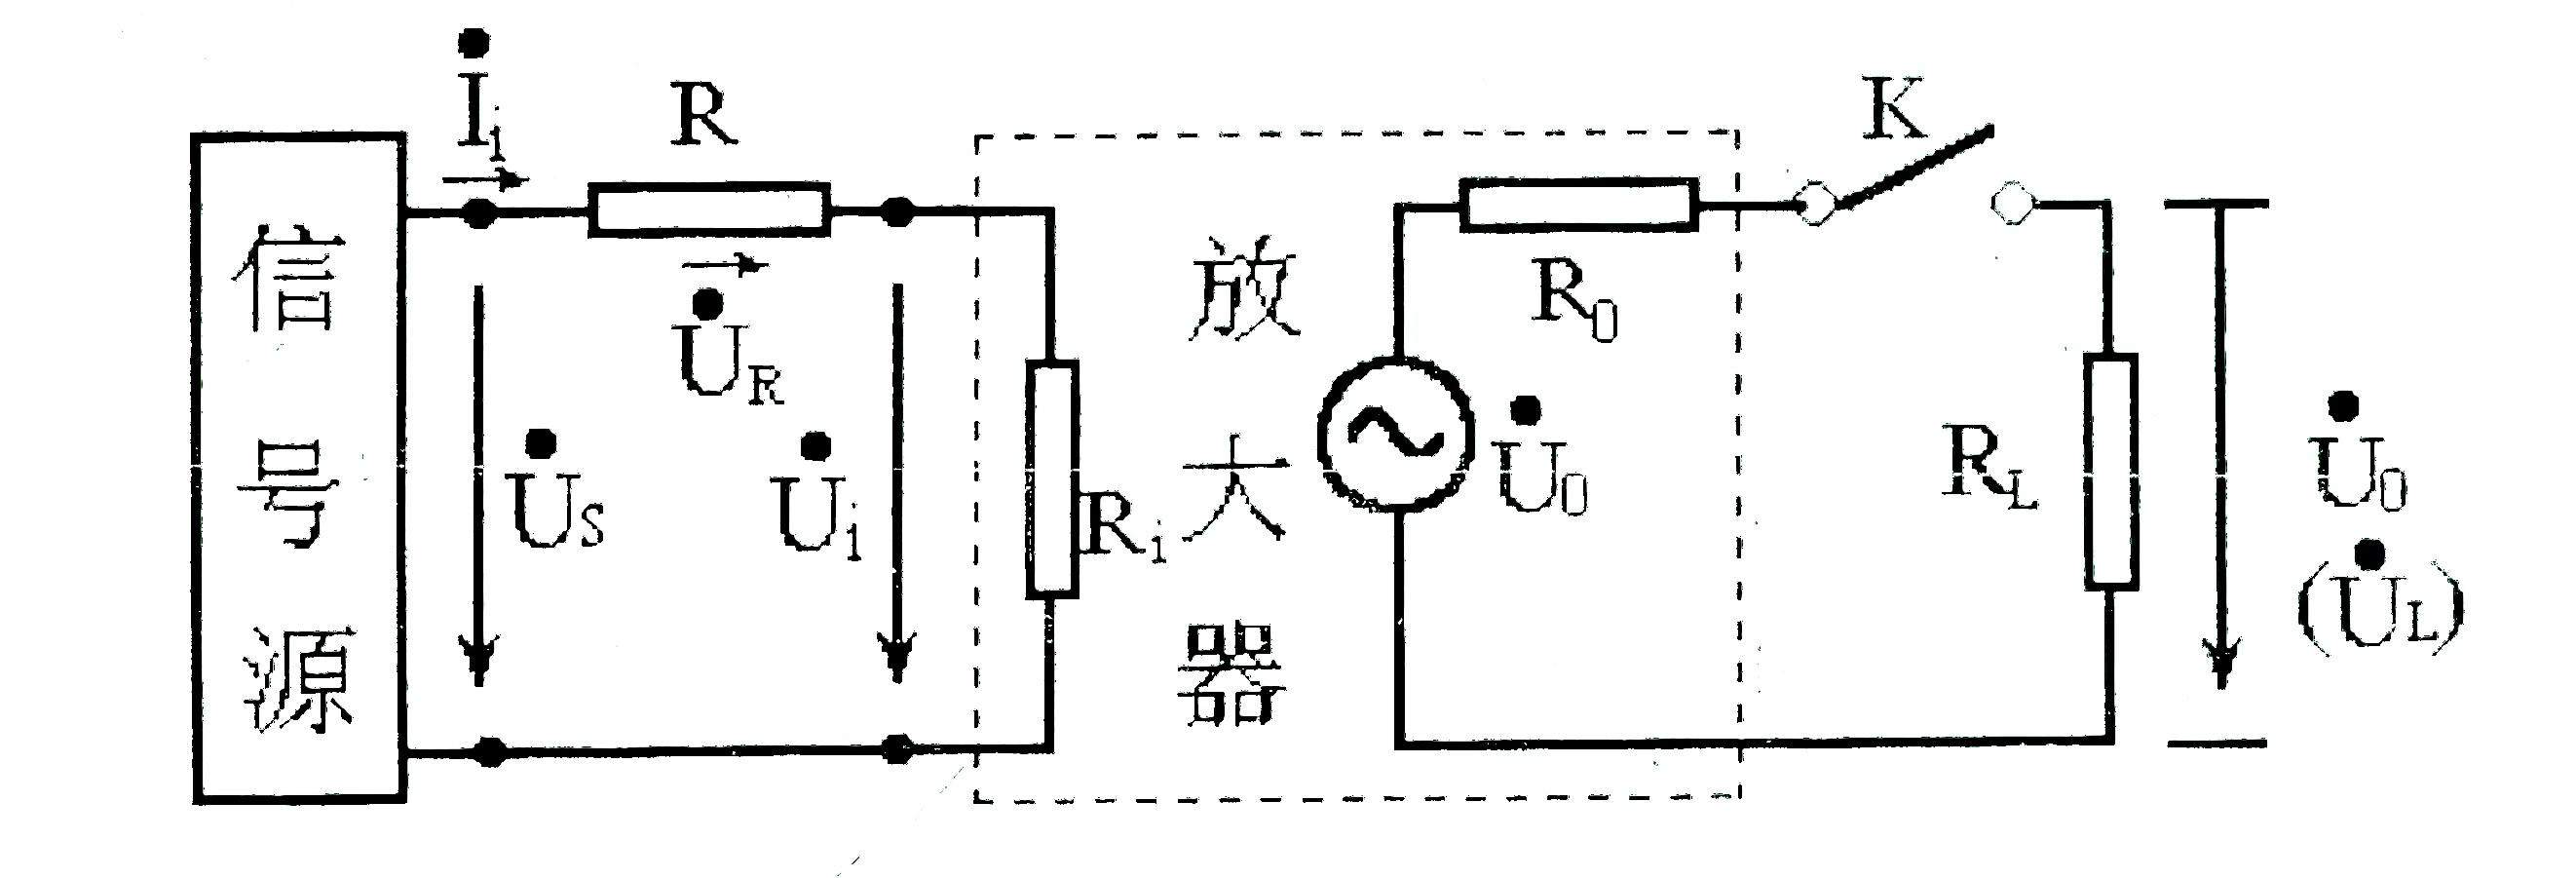
\includegraphics[height=80pt]{R}\\
        {\small 图四:实验电路}
    \end{center}

    \subsection{实验原理}\label{subsec:9}

    \subsection{实验内容}\label{subsec:10}

    \subsection{实验数据与误差分析}\label{subsec:11}

    \subsection{注意事项}\label{subsec:12}


    \section{测量幅频特性曲线}\label{sec:6}

    \subsection{实验原理}\label{subsec:13}
    \begin{center}
        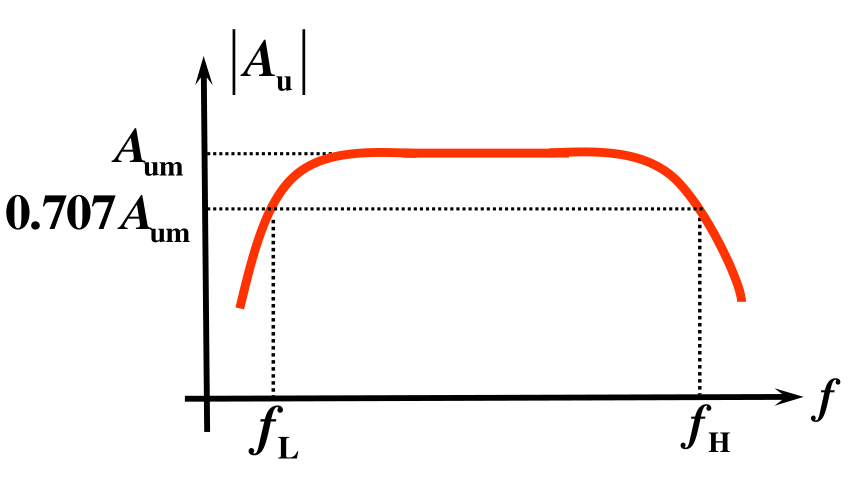
\includegraphics[height=120pt]{Af}\\
        {\small 图五:理想幅频特性曲线}
    \end{center}

    \subsection{实验内容}\label{subsec:14}

    \subsection{实验数据与误差分析}\label{subsec:15}
    \begin{center}
        \includegraphics[height=200pt]{Graph1}\\
        {\small 图六:实际幅频特性曲线}
    \end{center}

    \subsection{注意事项}\label{subsec:16}


    \section{观察静态工作点对输出波形失真的影响}\label{sec:7}

    \subsection{实验原理}\label{subsec:17}
    \begin{figure*}[htb]
        \centering
        \subfloat[饱和失真与截止失真]{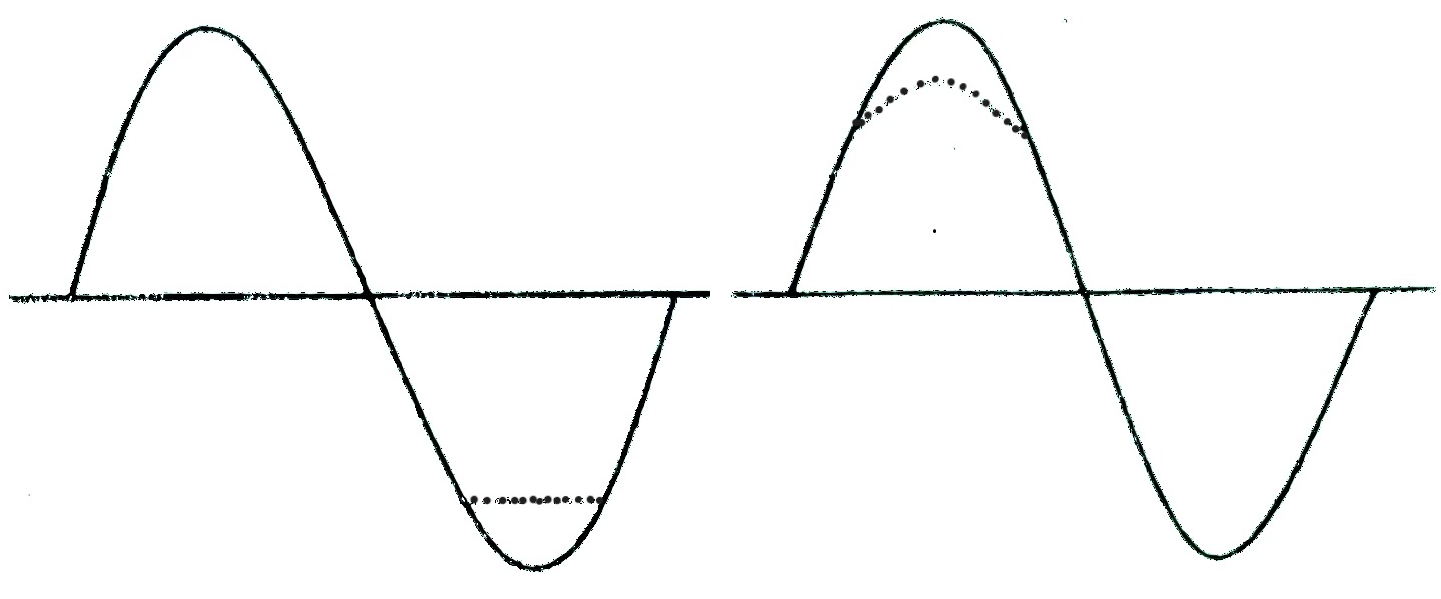
\includegraphics[height=100pt]{ID2}}
        \subfloat[电路参数对静态工作点影响]{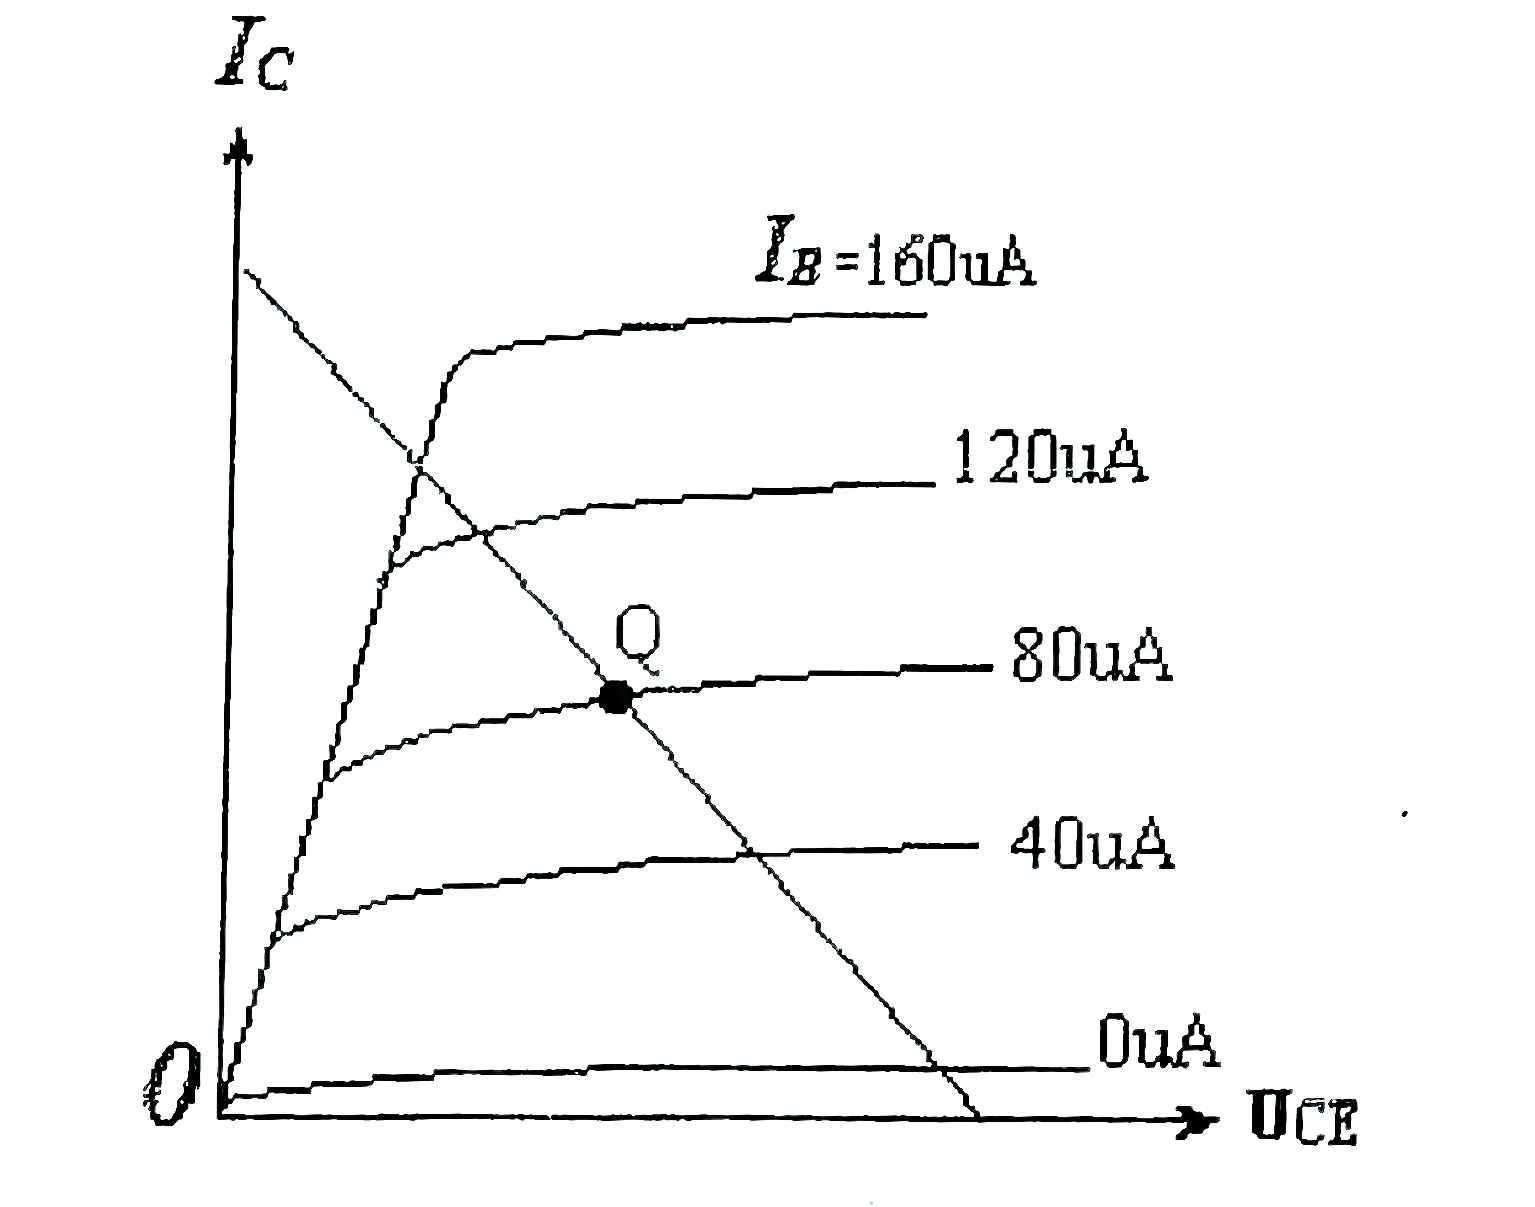
\includegraphics[height=100pt]{IU}}\\
        {\small 图七:理论图像}
    \end{figure*}

    \subsection{实验内容}\label{subsec:18}
    \begin{center}
        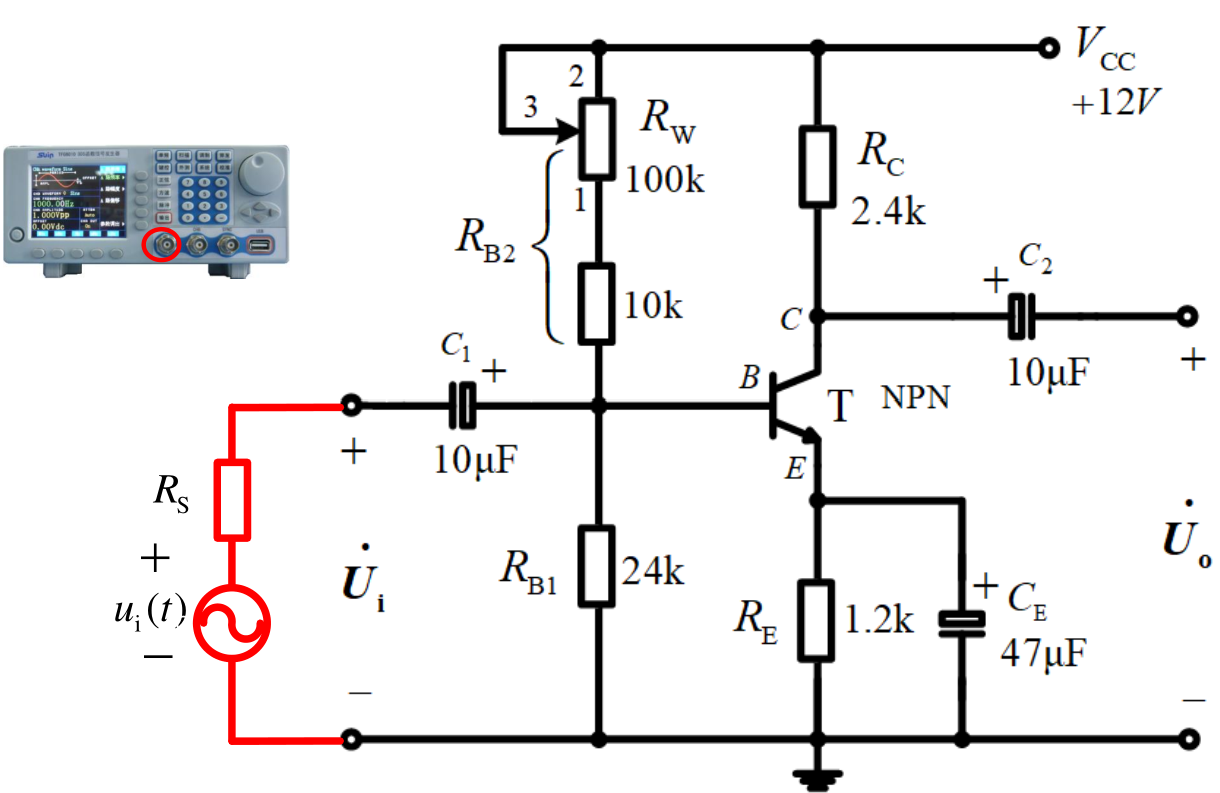
\includegraphics[height=150pt]{exp5}\\
        {\small 图八:实验电路}
    \end{center}

    \subsection{实验数据与误差分析}\label{subsec:19}
    \begin{figure*}[htb]
        \centering
        \subfloat[截止失真]{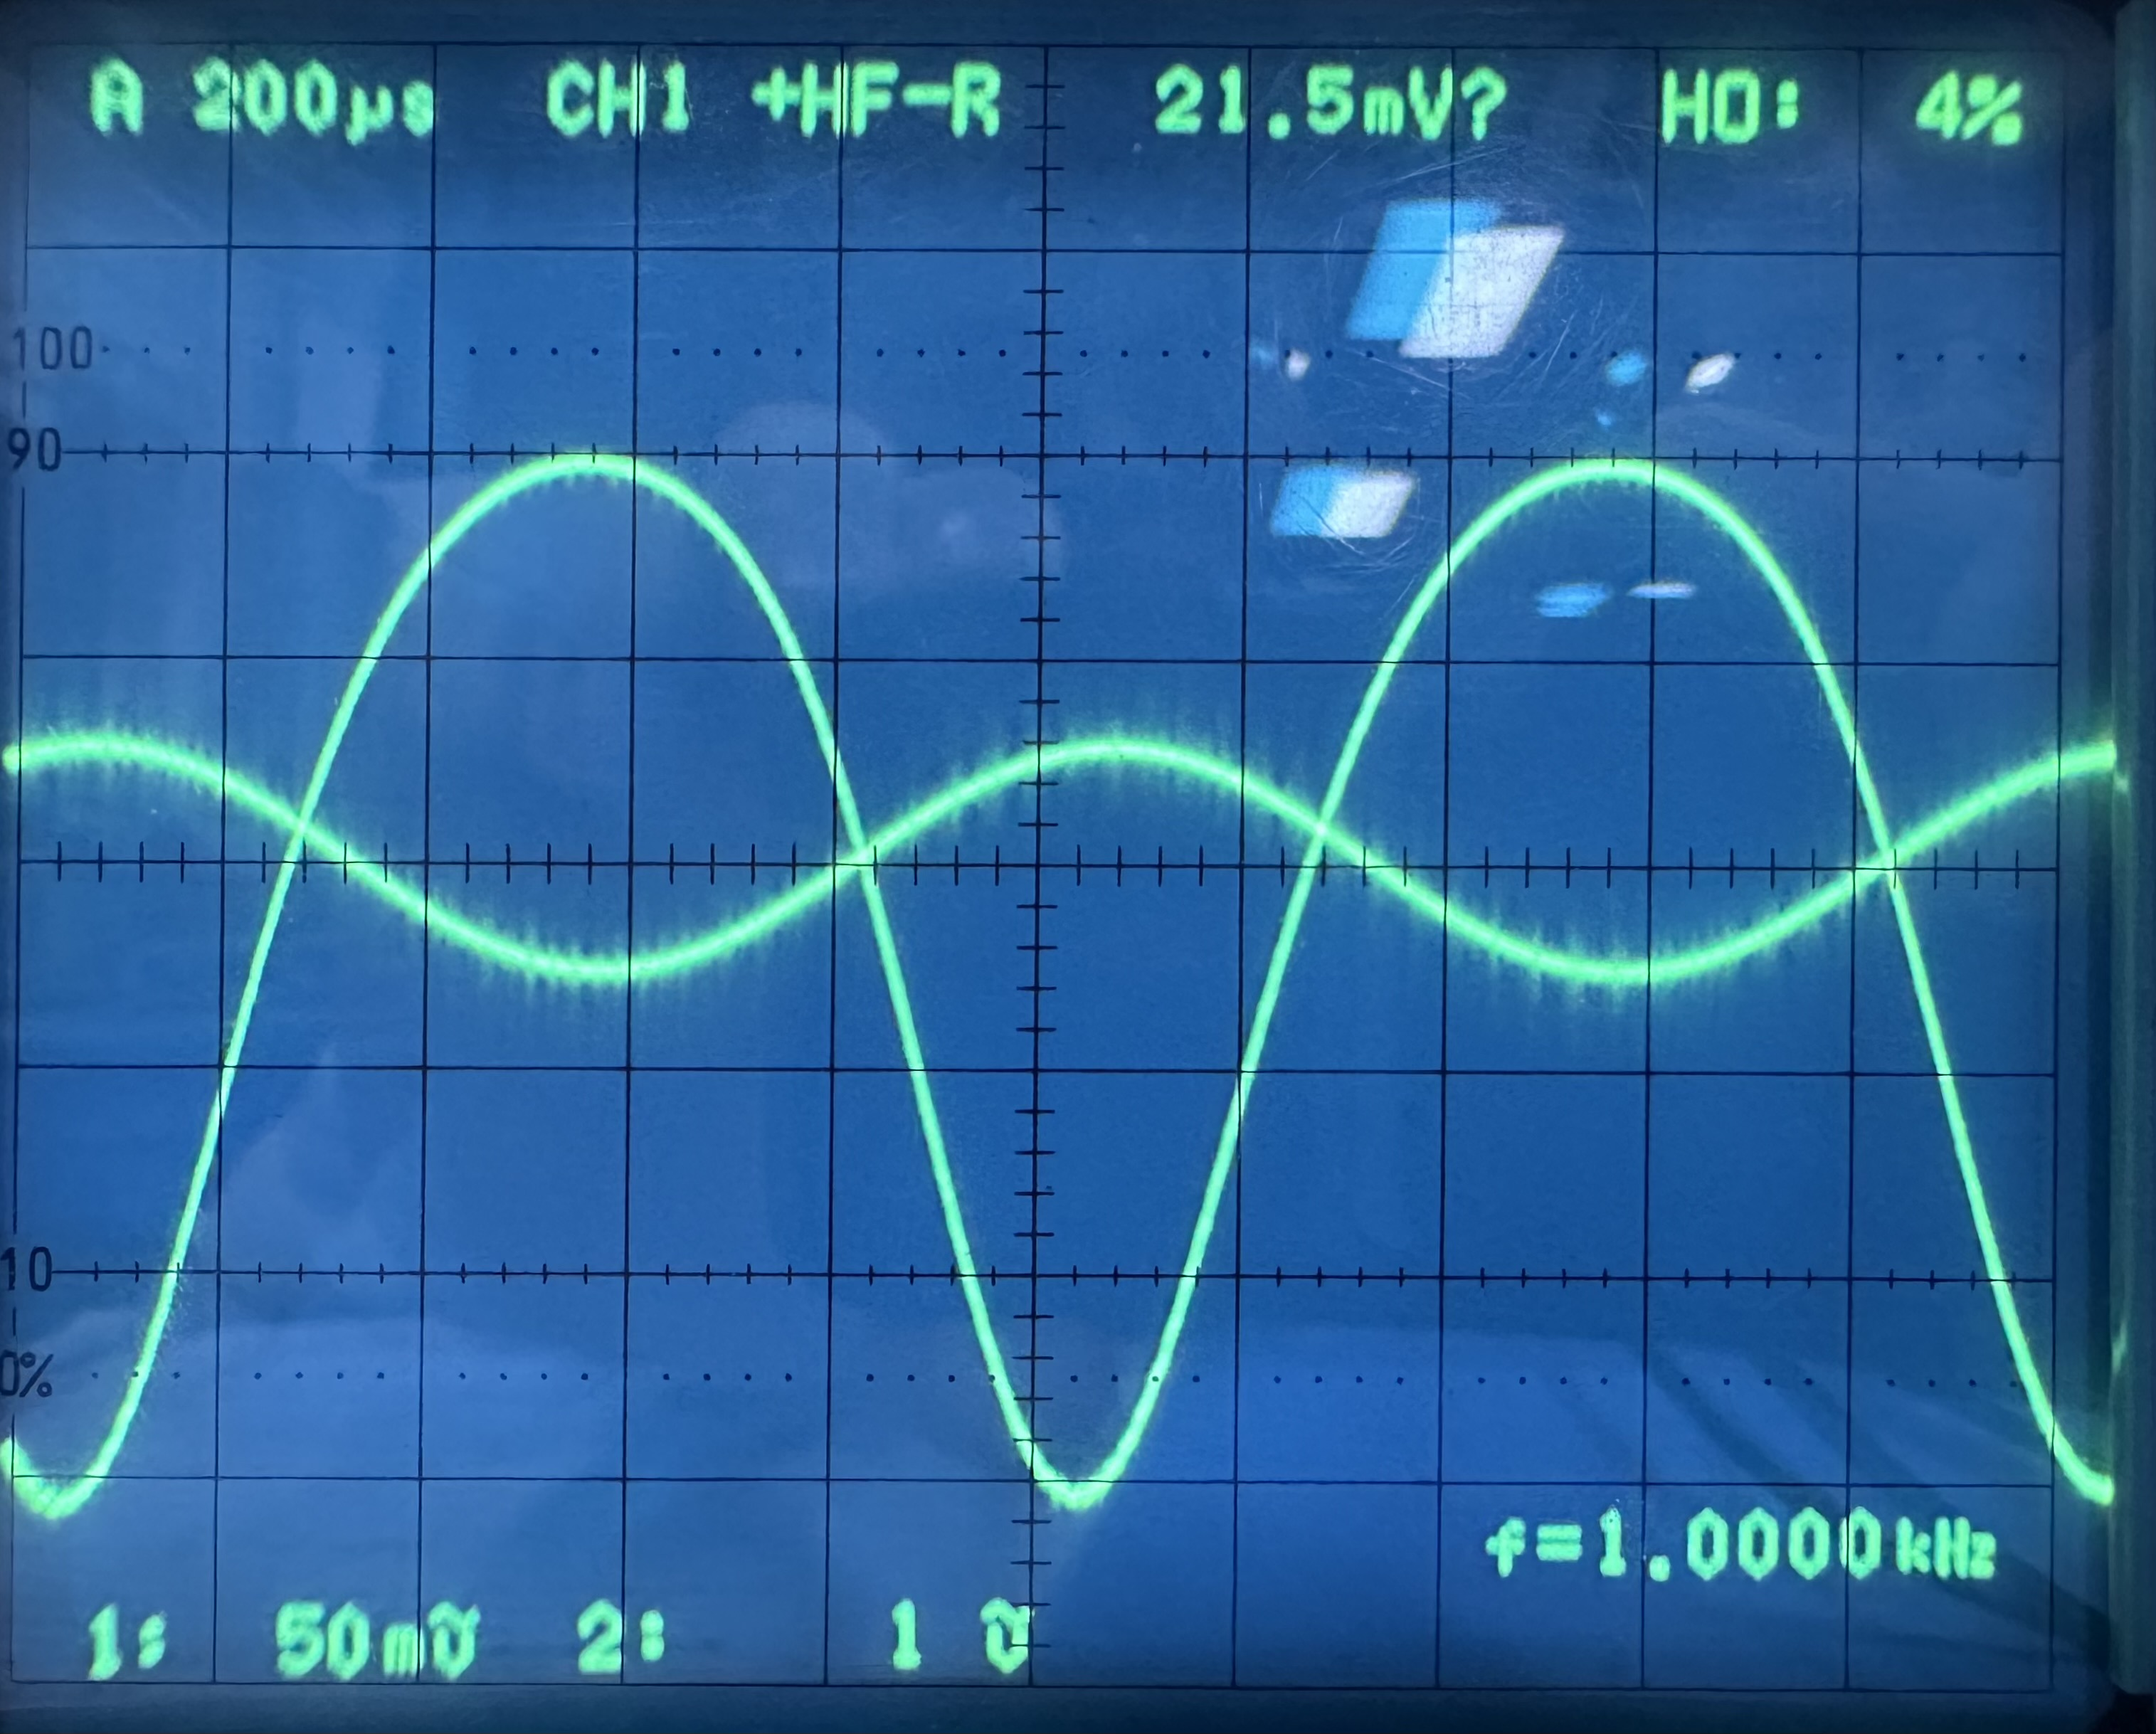
\includegraphics[height=120pt]{TD}}
        \subfloat[不失真]{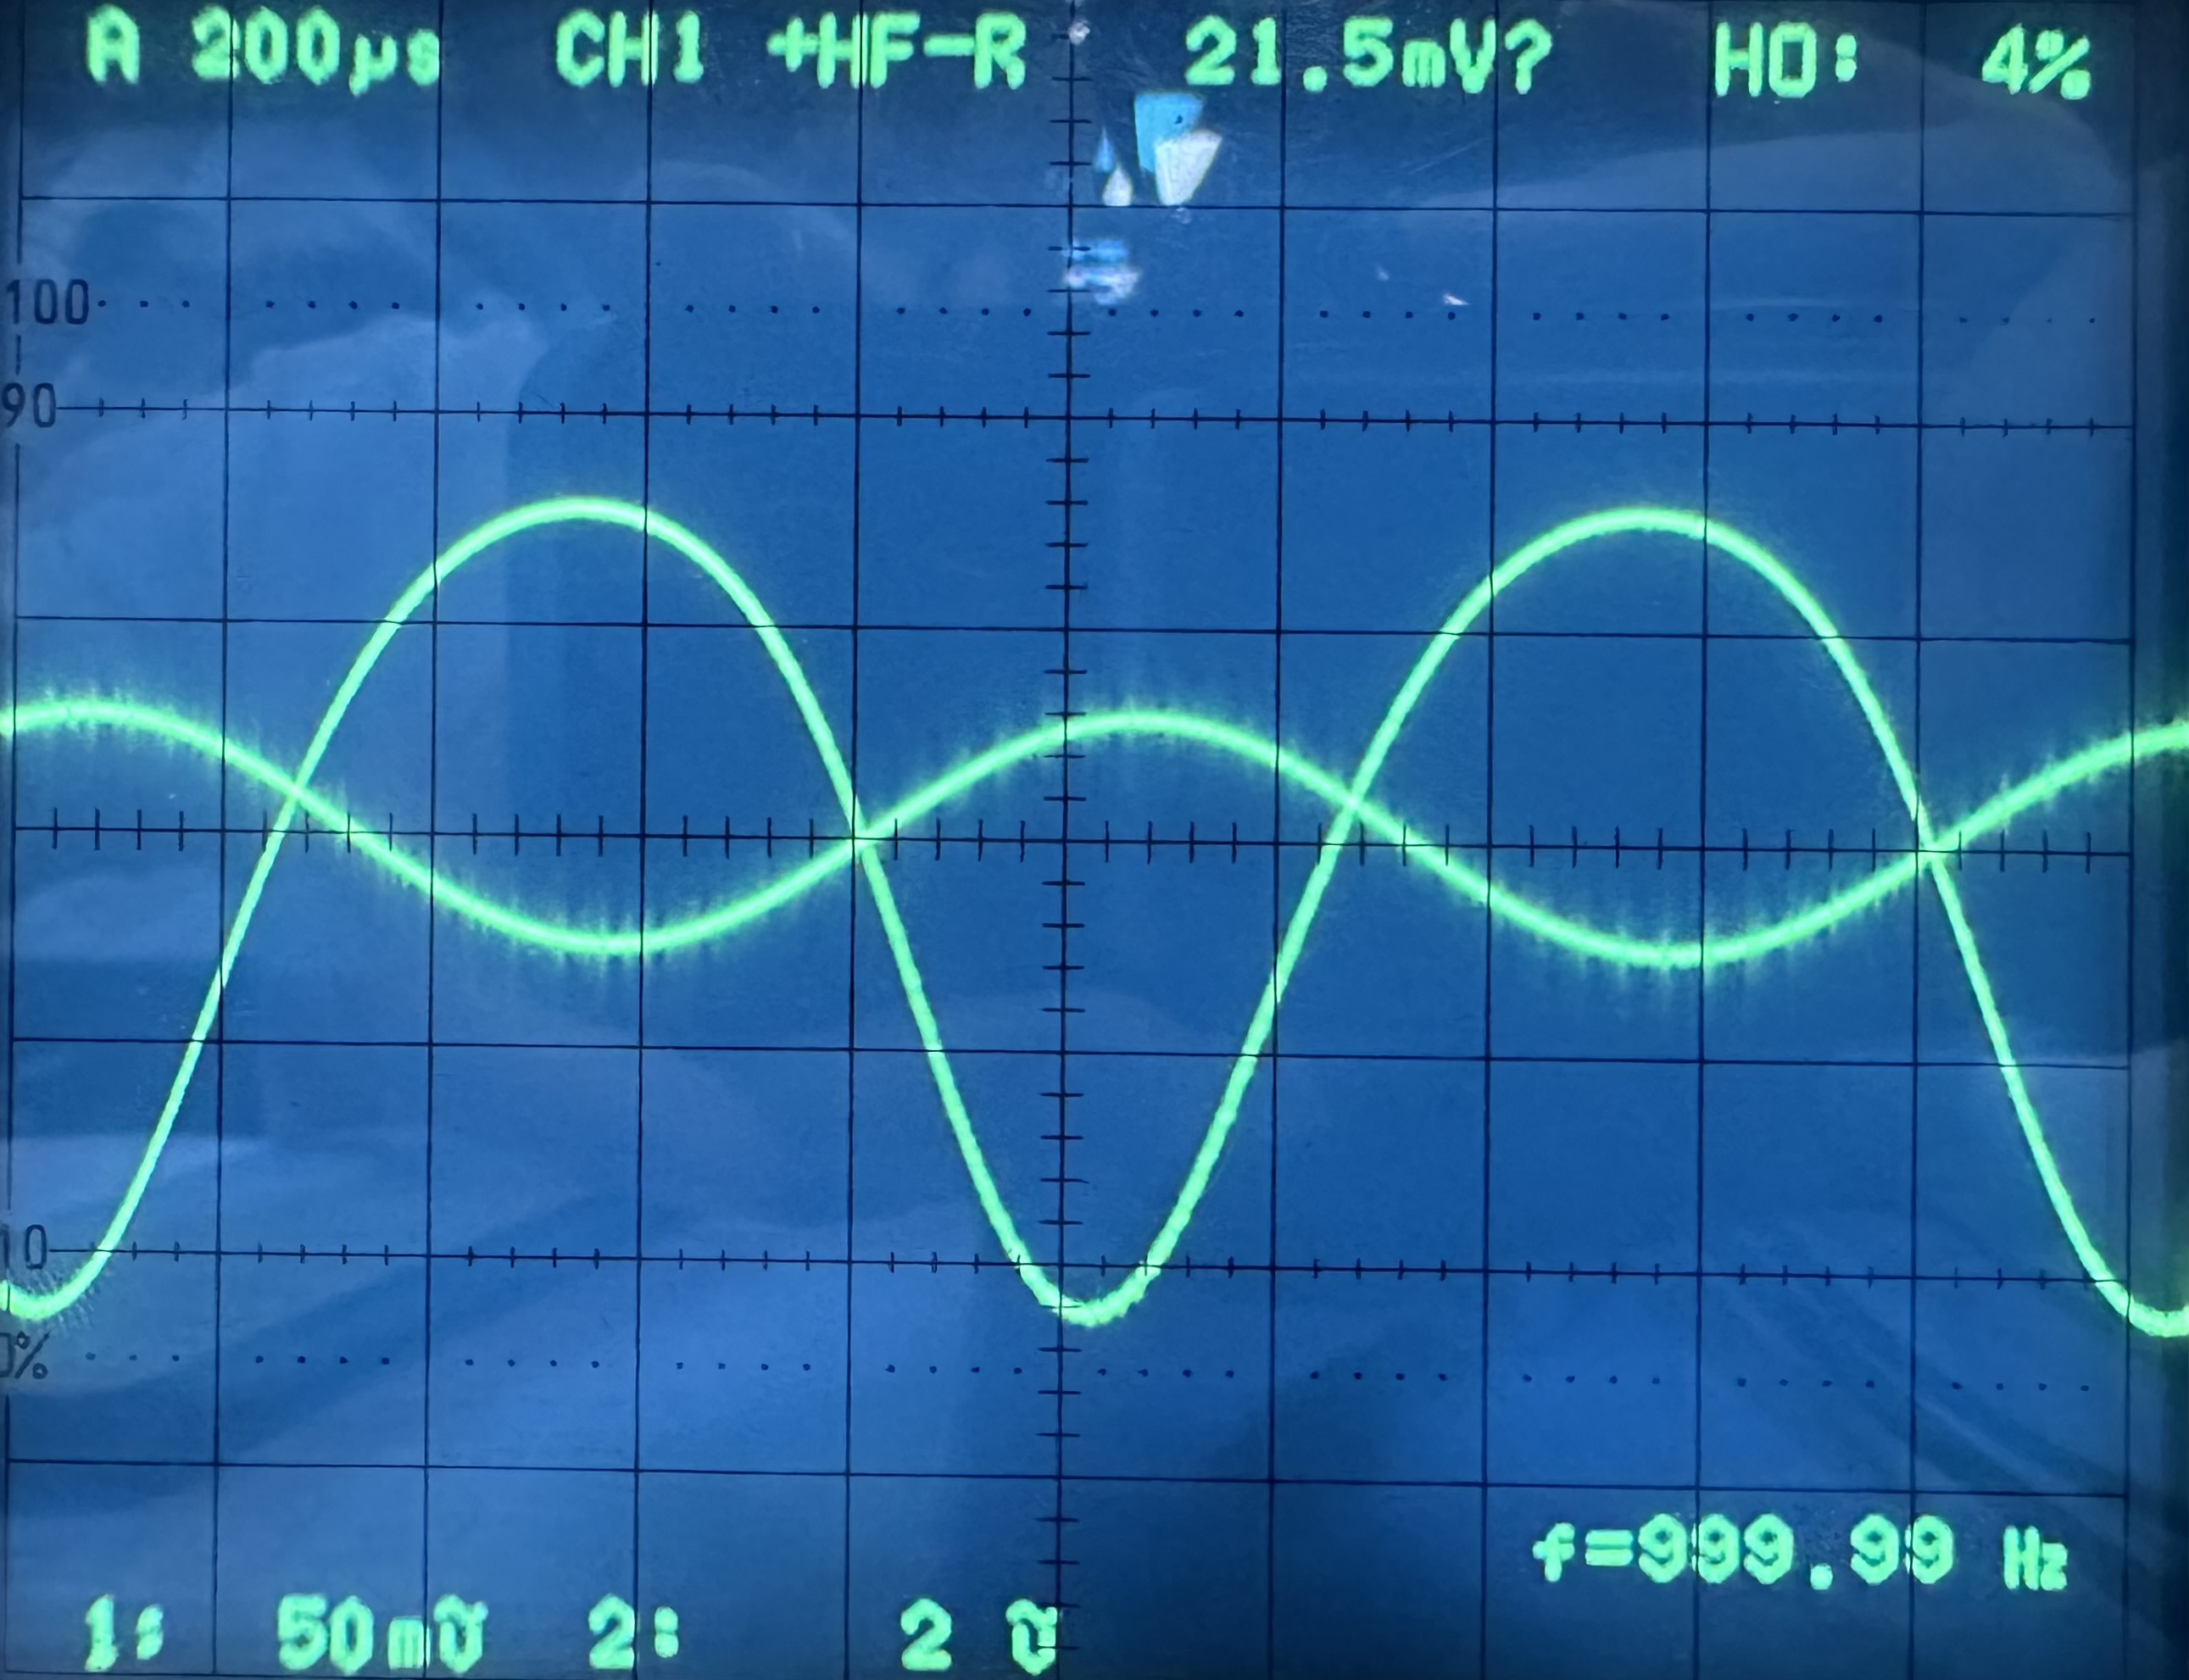
\includegraphics[height=120pt]{O}}
        \subfloat[饱和失真]{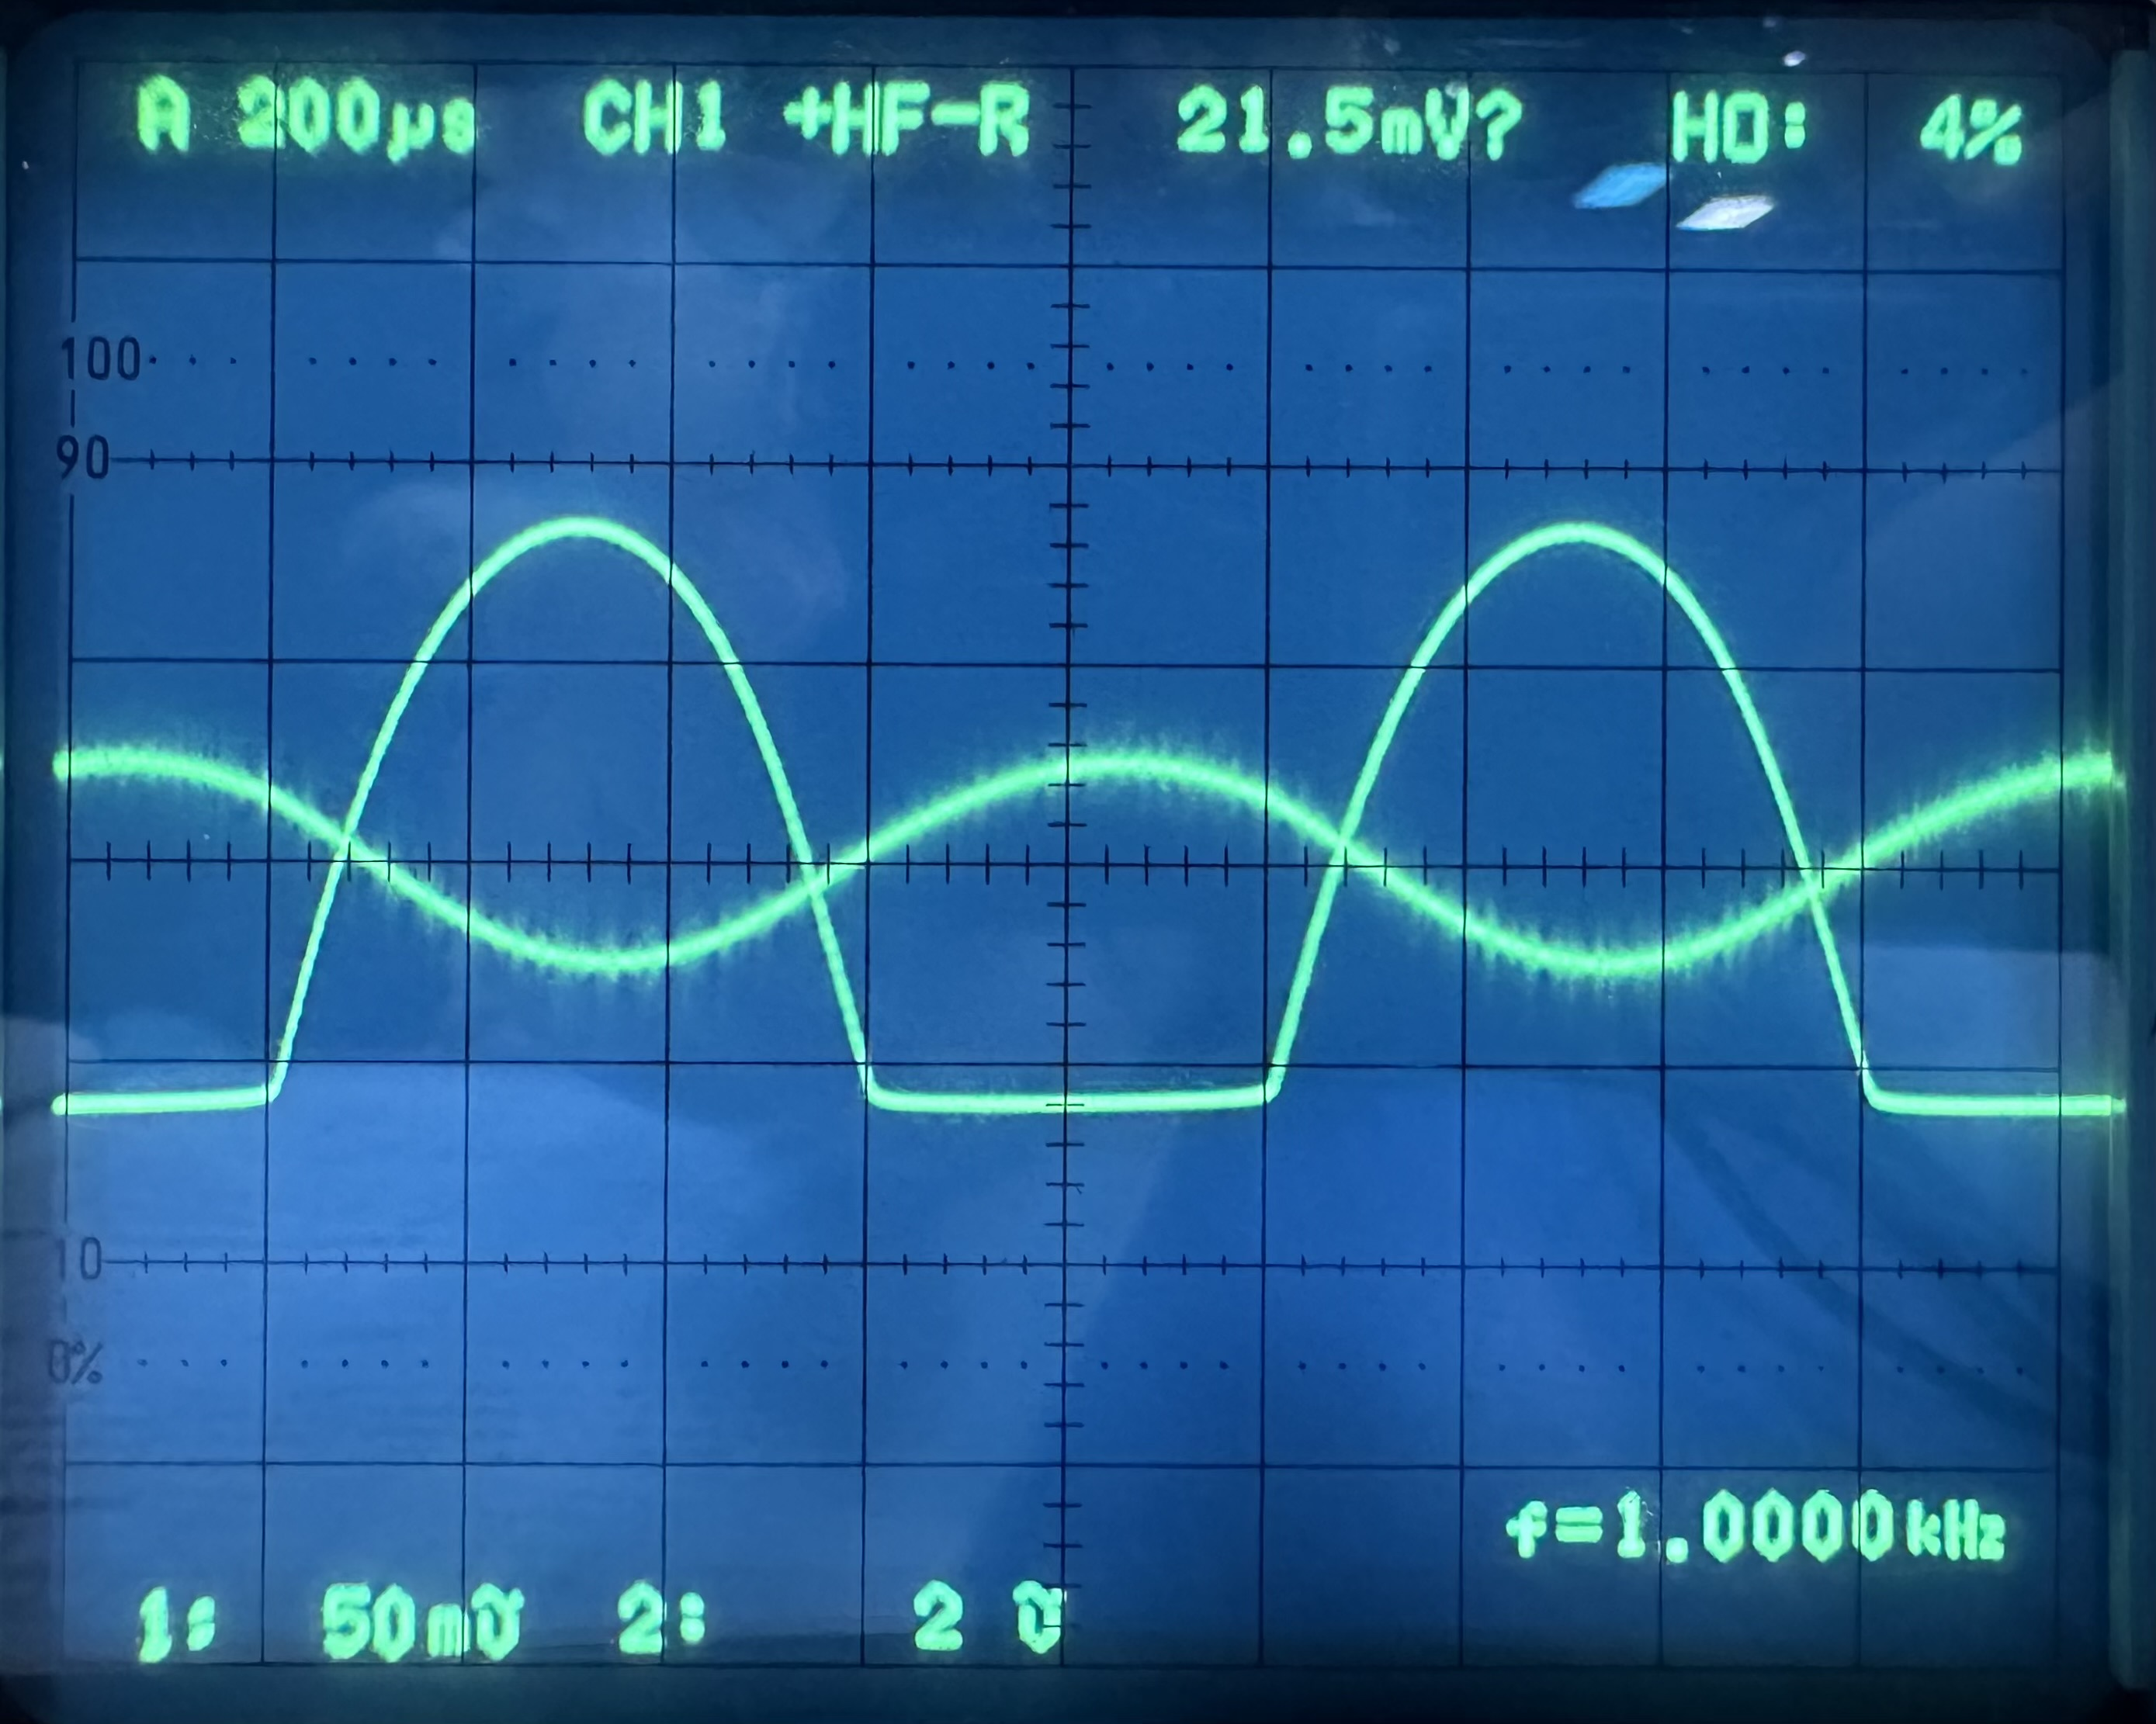
\includegraphics[height=120pt]{BD}}
        {\small 图九:输出波形失真图像}
    \end{figure*}

    \subsection{注意事项}\label{subsec:20}


    \section{思考题}\label{sec:8}


    \section{实验总结}\label{sec:9}

    \bibliography{main}
    \bibliographystyle{plain}

\end{document}
